\documentclass[11pt,a4paper]{article}

% ===================== Codificación y fuentes =====================
\usepackage[utf8]{inputenc}
\usepackage[T1]{fontenc}

% ===================== Página y utilidades ========================
\usepackage[left=2.5cm,right=2.5cm,top=2.1cm,bottom=2.1cm]{geometry}
\usepackage{array}
\usepackage{amsmath}
\usepackage{enumitem}
\usepackage{graphicx}
\usepackage{float}
\usepackage{xcolor}
\usepackage{titlesec}
\usepackage{fancyhdr}
\usepackage[most]{tcolorbox}

\usepackage{hyperref}
\usepackage{booktabs}
\usepackage{caption}
\captionsetup{font=small,skip=3pt}

% ===================== Etiquetas en español (sin babel) ===========
\renewcommand{\contentsname}{Índice}
\renewcommand{\figurename}{Figura}
\renewcommand{\tablename}{Tabla}
\renewcommand{\refname}{Bibliografía}

% ===================== Escala de grises (sin color) ================
\definecolor{negro}{RGB}{0,0,0}
\definecolor{gris}{RGB}{90,90,90}
\definecolor{grisclaro}{RGB}{150,150,150}
\definecolor{fillgray}{RGB}{175,175,175}

% ===================== Hipervínculos (negro) =======================
\hypersetup{colorlinks=true, linkcolor=negro, urlcolor=negro, citecolor=negro}

% ===================== Estilo de títulos ===========================
\titleformat{\section}{\large\bfseries\color{negro}}{\thesection.}{0.5em}{}
\titleformat{\subsection}{\normalsize\bfseries\color{negro}}{\thesubsection}{0.5em}{}
\titlespacing*{\section}{0pt}{0.9em}{0.3em}
\titlespacing*{\subsection}{0pt}{0.6em}{0.2em}

% ===================== Pie de página ===============================
\pagestyle{fancy}
\fancyhf{}
\fancyfoot[L]{\footnotesize\color{gris}Magíster en Ciencia de Datos e Inteligencia Artificial}
\fancyfoot[R]{\footnotesize\color{gris}\thepage}
\renewcommand{\headrulewidth}{0pt}
\renewcommand{\footrulewidth}{0.4pt}

% ===================== Datos del grupo ==============================
\newcommand{\proyTitulo}{Predicción de riesgo de enfermedad coronaria a 10 años}
\newcommand{\proyIntegrantes}{Felipe Díaz Toro, Pablo Ríos Passteni, Guillermo Subiabre Chacón, Ninoska Yévenes Hernández}
\newcommand{\proyDataset}{Framingham Heart Study (Riesgo Cardiovascular)}
\newcommand{\proyDocente}{Jean Paul Maidana}
\newcommand{\proyFecha}{14/10/2026}
\newcommand{\proyRepo}{\url{https://github.com/fdiaztoro/proyecto-grupo3-mcdi501}}

\setlength{\parindent}{0pt}
\setlength{\parskip}{0.2em}


\newcommand{\guia}[1]{{\small\itshape\color{gris}#1}\par\vspace{0.15em}}
\newcommand{\resp}[1]{{\footnotesize\itshape\color{gris}[\,Responsable: #1\,]}\par\vspace{0.3em}}
\newcommand{\desarrolle}{{\footnotesize\itshape\color{fillgray}[\,Desarrollar aquí\,]}\par\vspace{6em}}

% Caja de información de la evaluación (escala de grises):
\newtcolorbox{infobox}[1][Información de la evaluación]{colback=black!3,colframe=negro,
  fonttitle=\bfseries,coltitle=white,title={#1},boxrule=0.6pt,arc=1pt,
  left=8pt,right=8pt,top=3pt,bottom=3pt,breakable}

% Caja de conexión con evaluaciones previas (gris, sin color):
\newtcolorbox{conexionbox}[1][Conexión con evaluaciones anteriores]{colback=black!6,colframe=gris,
  fonttitle=\bfseries,coltitle=white,title={#1},boxrule=0.6pt,arc=1pt,
  left=8pt,right=8pt,top=3pt,bottom=3pt,breakable}

\begin{document}
\pagenumbering{gobble}

\thispagestyle{empty}
\begin{center}
\vspace*{1.0cm}

\includegraphics[height=4.4cm]{logo_unab.png}\\[1.3cm]

{\footnotesize\color{gris}\MakeUppercase{Magíster en Ciencia de Datos e Inteligencia Artificial}}\\[0.15cm]
{\footnotesize\color{grisclaro}MCDI501: Estadística Computacional para la Toma de Decisiones}\\[2.0cm]

{\Large\bfseries\color{negro} Evaluación Sumativa 2}\\[0.45cm]
{\large\color{negro} Validación, Simulación y Métodos de Remuestreo}\\[1.0cm]

{\Large\bfseries\color{negro} \proyTitulo}\\[0.4cm]
{\normalsize\color{gris} Framingham Heart Study}\\[0.8cm]

{\small\itshape\color{gris} Informe técnico grupal \textperiodcentered\ Grupo 3 \textperiodcentered\ 20\,\%}
\end{center}

\vspace{1.6cm}

\begin{flushleft}
\setlength{\extrarowheight}{5pt}
\begin{tabular}{@{}>{\bfseries\color{negro}}l >{\raggedright\arraybackslash}p{11cm}@{}}
Título del proyecto: & \proyTitulo \\
Integrantes:         & \proyIntegrantes \\
Dataset:             & \proyDataset \\
Docente:             & \proyDocente \\
Fecha:               & \proyFecha \\
Repositorio GitHub:  & \proyRepo \\
\end{tabular}
\end{flushleft}

\clearpage
\pagenumbering{arabic}
\begin{infobox}
\textbf{Fase del proyecto:} Fase 3: Desarrollo del proyecto\\
\textbf{Modalidad:} Grupal\qquad\textbf{Ponderación:} 20\,\% de la nota final\\
\textbf{Entregables:} Informe PDF (máx.\ 7 págs.)\ \textperiodcentered\ Notebook \texttt{.ipynb}\ \textperiodcentered\ Repositorio GitHub (carpetas S1, S2 y archivo de resultados validados)\\
\textbf{Resultado de aprendizaje (RA2):} implementar métodos computacionales de simulación y remuestreo para apoyar la toma de decisiones en escenarios complejos.\\
\textbf{Indicadores:} ID2.1, ID2.2, ID2.3.\\
\textbf{Prerrequisito:} Sumativa 1 completada (usarán sus resultados).
\end{infobox}
\begin{conexionbox}
Esta evaluación \textbf{no es independiente}: todo el trabajo se construye explícitamente sobre los resultados de la Sumativa 1 (parámetros estimados, intervalos de confianza, pruebas de hipótesis y correlaciones).
\end{conexionbox}

\vspace{0.1em}
\tableofcontents

\noindent Esta evaluación valida con remuestreo y simulación los resultados de la Sumativa 1 (S1) sobre el Framingham Heart Study (Dileep, s.f.; $n=4.238$; variable objetivo \texttt{TenYearCHD}, con 15,2\,\% de casos). Todo parte de los resultados de S1; no se usan datos ni parámetros externos. Semilla 42, $B=10.000$ en todos los procedimientos, implementados con NumPy, pandas y SciPy (Harris et~al., 2020; McKinney, 2010; Virtanen et~al., 2020).

% ===================================================================
% Responsable: Ninoska Yévenes
\section{Validación de resultados de S1 mediante bootstrap}

Se remuestrearon con reposición las filas disponibles de cada variable ($B=10.000$) para cuatro parámetros de S1 (edad, colesterol y presión sistólica medias, y proporción de CHD) más la mediana del colesterol, que no tiene IC clásico. Se calcularon los IC percentil y BCa (Efron, 1987), este último implementado a mano (sesgo $z_0$ y aceleración $a$ por jackknife) y contrastado con \texttt{scipy.stats.bootstrap}. El clásico es el de S1 (t de Student; Wilson para la proporción).

\begin{table}[H]
\centering
\small
\caption{IC al 95\,\% de los parámetros de S1: clásico, percentil y BCa.}
\label{tab:boot}
\begin{tabular}{lrccc}
\toprule
\textbf{Parámetro} & \textbf{Est.} & \textbf{Clásico (S1)} & \textbf{Percentil} & \textbf{BCa} \\
\midrule
Edad media (años)           & 49,59  & [49,33; 49,84]   & [49,33; 49,85]   & [49,33; 49,85] \\
Colesterol medio (mg/dL)    & 236,72 & [235,37; 238,07] & [235,39; 238,07] & [235,41; 238,08] \\
Presión sistólica (mmHg)    & 132,35 & [131,69; 133,02] & [131,70; 133,01] & [131,71; 133,03] \\
Proporción de CHD (\%)      & 15,20  & [14,15; 16,31]   & [14,13; 16,30]   & [14,13; 16,30] \\
Mediana colesterol (mg/dL)  & 234    & ---              & [232; 235]       & [232; 236] \\
\bottomrule
\end{tabular}
\end{table}

\begin{figure}[H]
\centering
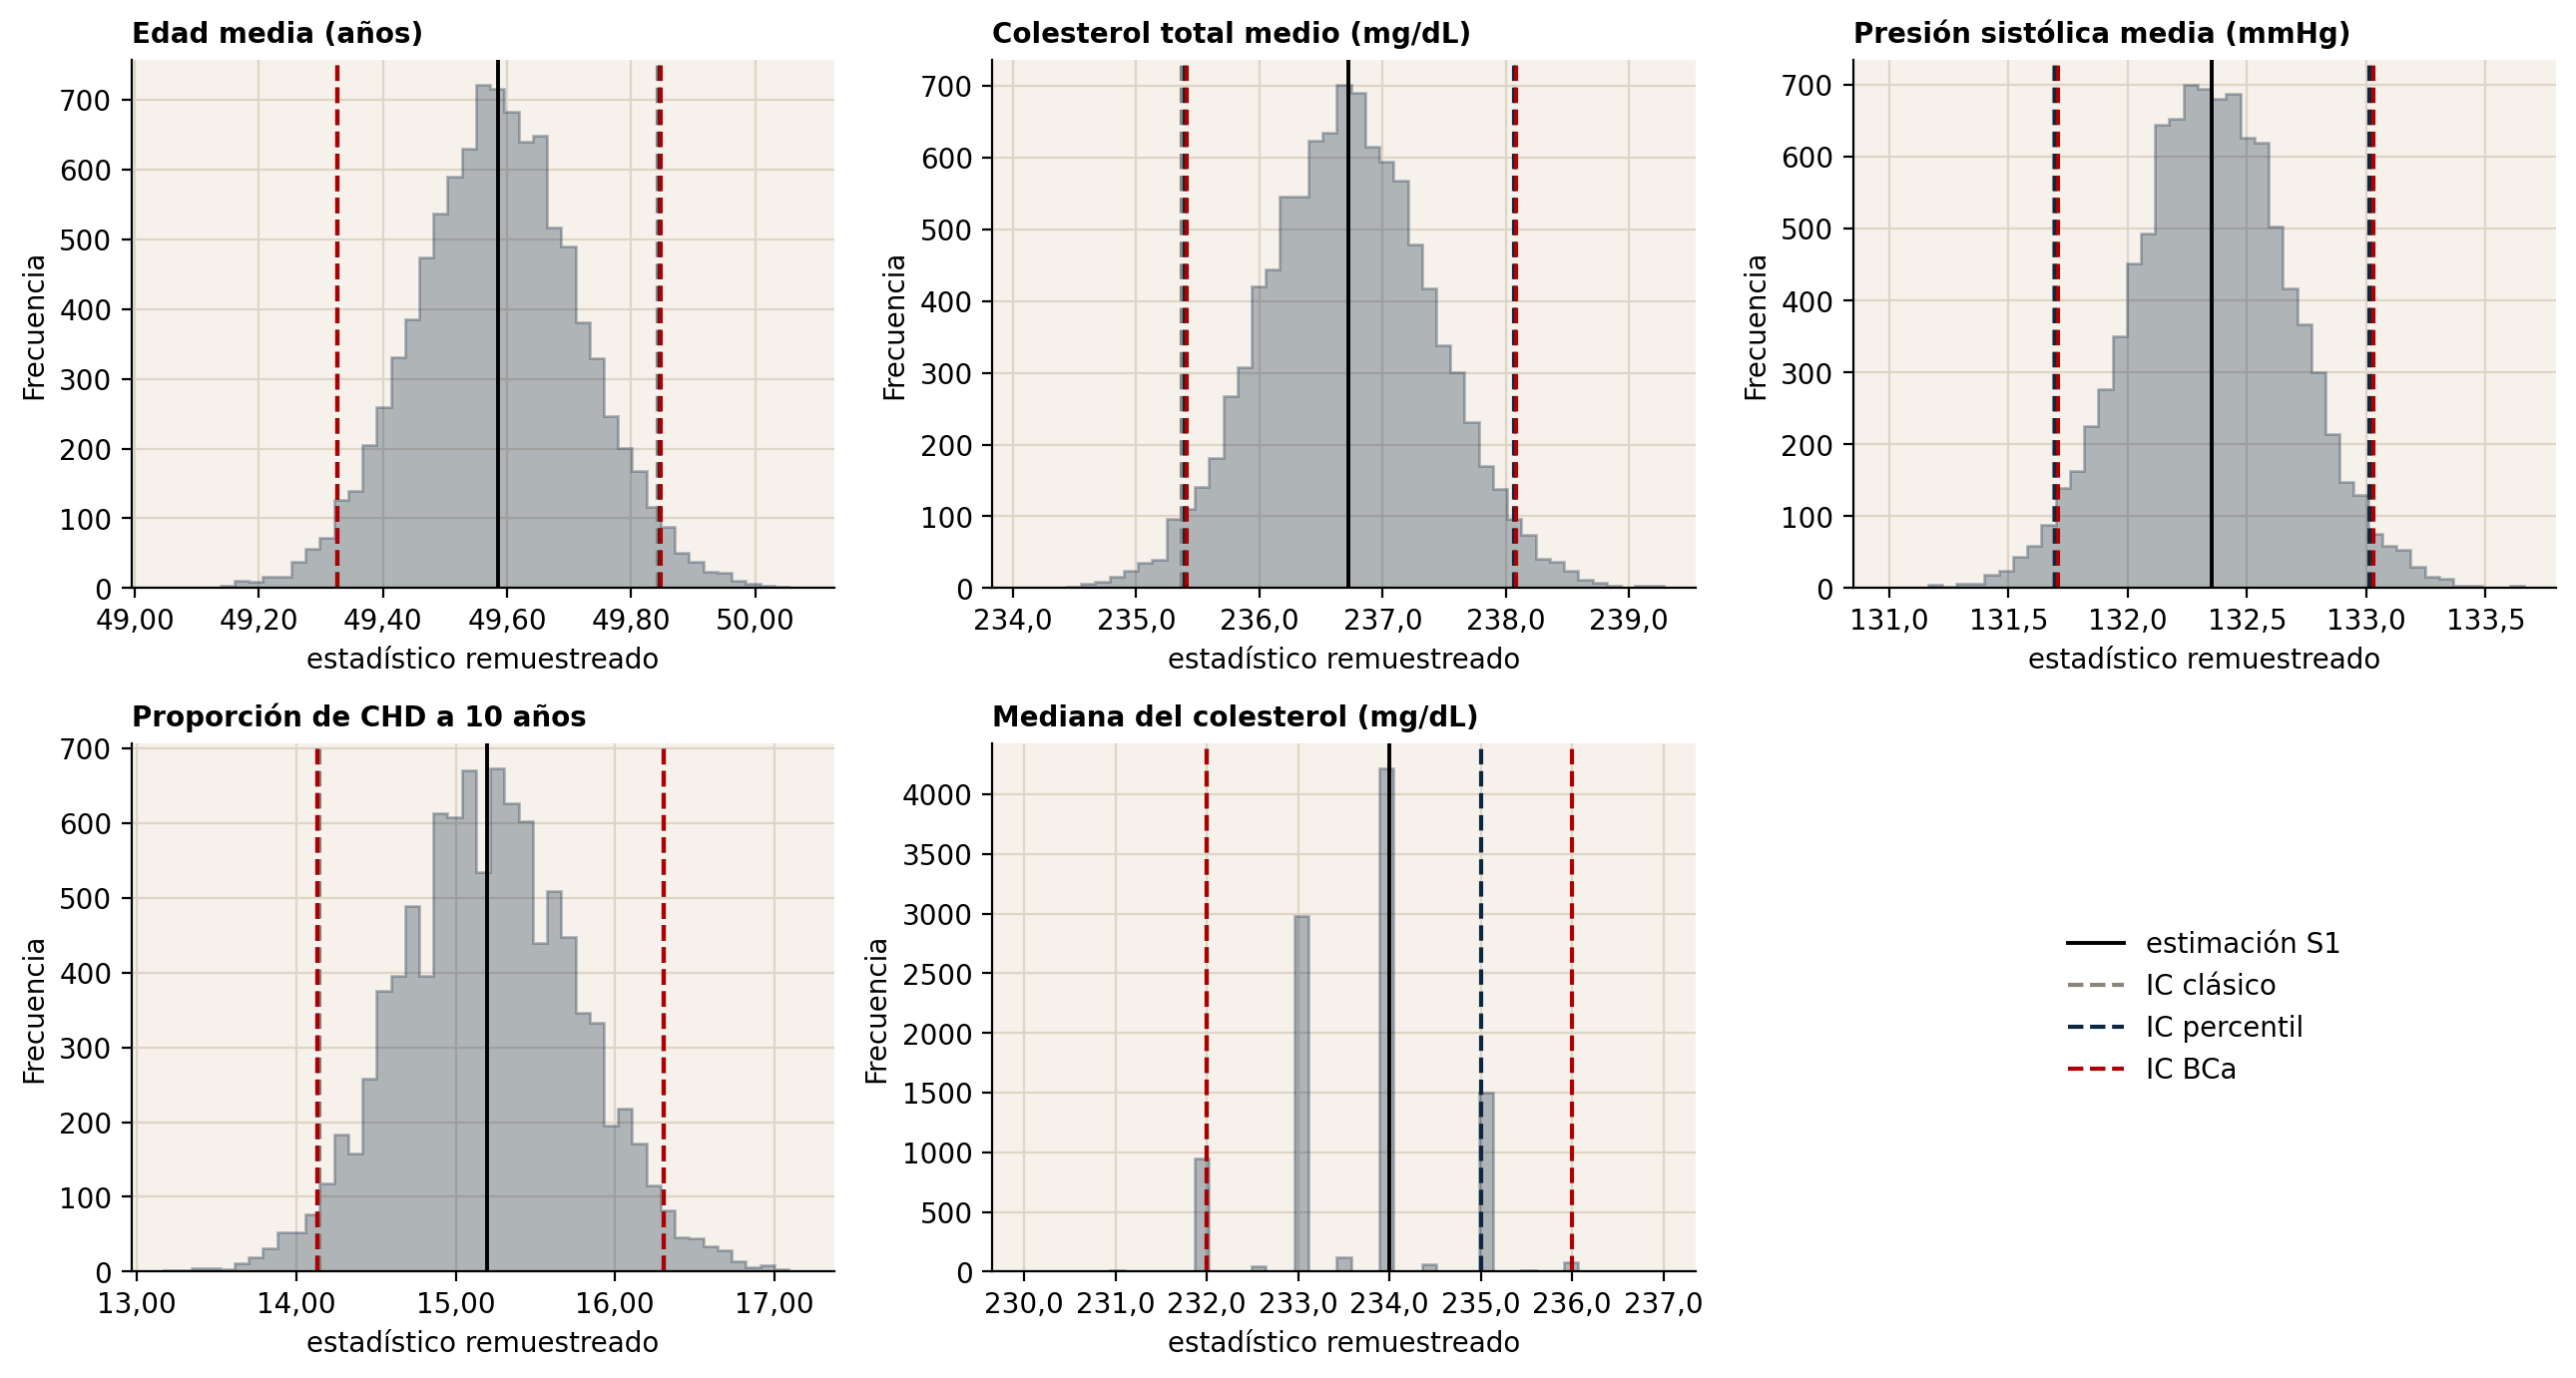
\includegraphics[width=0.8\linewidth]{figuras/fig_bootstrap.png}
\caption{Distribución bootstrap de los parámetros y sus intervalos.}
\label{fig:boot}
\end{figure}

\textbf{Discrepancias.} En las tres medias y en la proporción, los tres intervalos prácticamente coinciden: los límites difieren en centésimas y el BCa se aparta del clásico entre 0,6\,\% y 1,4\,\% de su amplitud. Los factores de corrección son pequeños ($|z_0|\leq0{,}012$; $a\leq0{,}005$): con unas 4.200 observaciones el Teorema Central del Límite ya opera, incluso en el colesterol (asimetría 0,87), y casi no hay sesgo ni asimetría que corregir. El BCa propio y el de SciPy difieren en menos de 1,5\,\% de la amplitud, lo que valida la implementación. La mediana es el caso aparte: como el colesterol se mide en enteros, su distribución bootstrap toma pocos valores distintos, el jackknife queda degenerado ($a=0$) y SciPy no logra calcular el BCa; sus intervalos son toscos y se informan con cautela.

\textbf{Interpretación y supuestos.} El 95\,\% describe el \emph{procedimiento}, no un intervalo en particular: si se repitiera el muestreo muchas veces y en cada muestra se construyera un intervalo con el mismo método, cerca del 95\,\% de esos intervalos contendría el valor verdadero del parámetro, que es fijo; no se afirma que un intervalo concreto lo contenga con probabilidad 0,95. El método clásico exige una media aproximadamente normal e independencia; el percentil supone una distribución bootstrap simétrica y sin sesgo; el BCa corrige ambos, pero es más costoso y sensible a valores extremos (Efron y Tibshirani, 1993; Maidana, 2026). Como los tres coinciden, los intervalos de S1 quedan validados; la independencia entre participantes sigue siendo un supuesto que ningún método comprueba.

% ===================================================================
% Responsable: Ninoska Yévenes
\section{Validación de pruebas de hipótesis mediante permutación}

Se validaron las dos pruebas de S1 con 10.000 permutaciones de las etiquetas de CHD, que bajo $H_0$ son intercambiables (sin supuestos de distribución). (i) \emph{Edad y CHD}: la diferencia de medias observada es de 5,38 años (t de Welch = 15,58). (ii) \emph{Hipertensión prevalente y CHD}: $\chi^2=133{,}7$ sin corrección ($132{,}6$ con Yates, el valor de S1). El valor $p$ se calculó como $(1+\#\{\text{estadístico permutado}\geq\text{observado}\})/(B+1)$, de modo que no puede ser cero (Phipson y Smyth, 2010).

\begin{figure}[H]
\centering
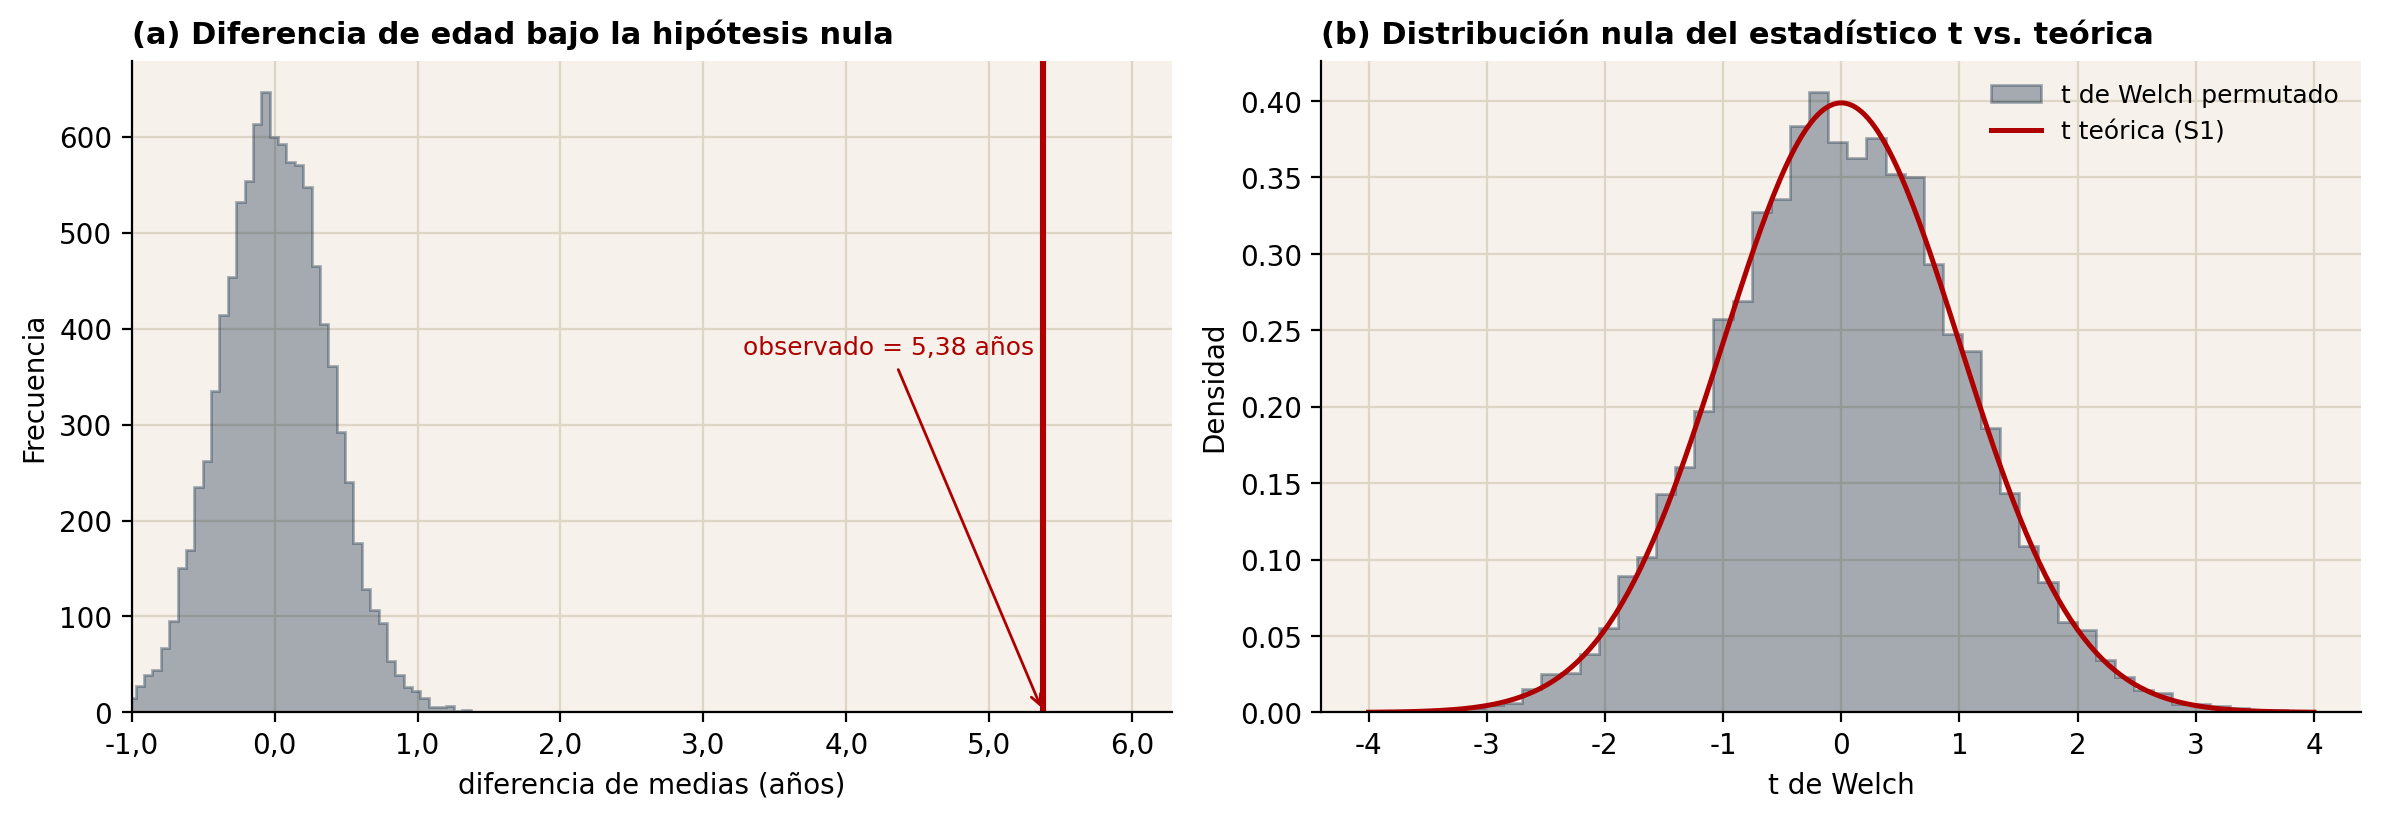
\includegraphics[width=\linewidth]{figuras/fig_permutacion.png}
\caption{Distribución nula permutada y valor observado (línea) en las dos pruebas.}
\label{fig:perm}
\end{figure}

\textbf{Concordancia.} Ninguna de las 10.000 permutaciones alcanza el valor observado en ninguna prueba, por lo que $p=0{,}0001$ en ambas, la cota mínima posible $1/(B+1)$. Los valores paramétricos de S1 ($1{,}0\times10^{-48}$ y $1{,}1\times10^{-30}$) son órdenes de magnitud menores, pero no son comparables en tamaño: la permutación no puede informar valores menores que $1/(B+1)$. Ambos enfoques coinciden en la decisión, que es rechazar $H_0$. Además, la distribución que supone la prueba de S1 describe bien los datos permutados: el t de Welch permutado tiene media 0,004 y desviación estándar 1,009, con cuantiles 2,5\,\% y 97,5\,\% de $-1{,}95$ y $2{,}00$ (teóricos $\pm1{,}96$); y el $\chi^2$ permutado tiene media 1,003 y cuantil 95\,\% de 3,78 (teóricos 1 y 3,84).

\textbf{Cuál es más apropiado.} Con $n=4.238$ y grupos desiguales (644 casos y 3.594 sin CHD) la prueba de Welch (1947) es adecuada y entrega un valor $p$ más informativo; la permutación actúa como confirmación libre de supuestos de distribución. Ambas suponen independencia entre participantes.

% ===================================================================
% Responsable: Guillermo Subiabre
\section{Evaluación de estabilidad de correlaciones}

Se eligieron cinco correlaciones relevantes de S1 y se calculó su IC bootstrap al 95\,\% (10.000 remuestras de filas completas, método percentil), contrastado con el IC de Fisher (1915). Se llama \emph{robusta} a la correlación cuyo intervalo es estrecho y excluye el cero, e \emph{inestable} a la que lo incluye.

\begin{figure}[H]
\centering
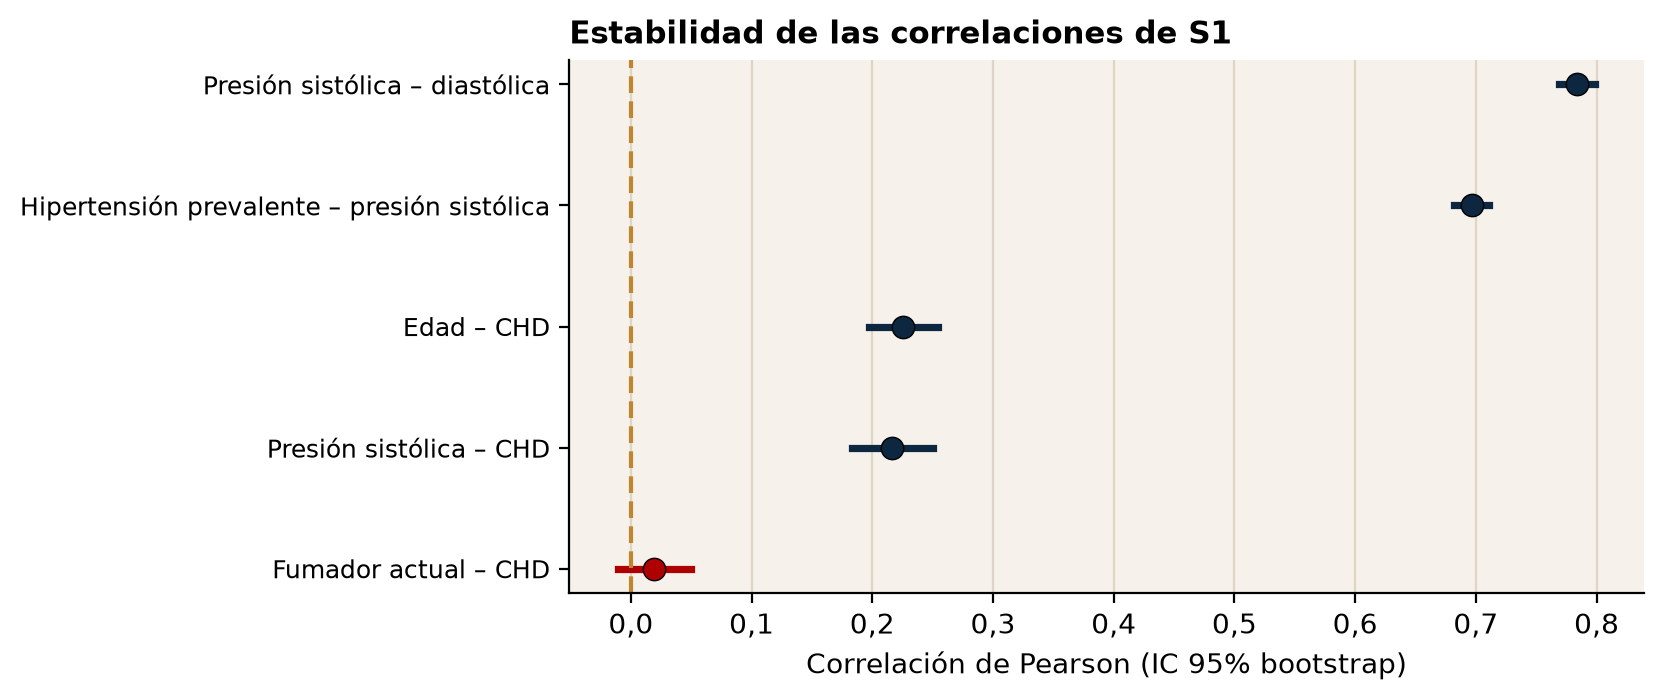
\includegraphics[width=0.78\linewidth]{figuras/fig_correlaciones.png}
\caption{Correlaciones de S1 con su IC bootstrap al 95\,\%.}
\label{fig:corr}
\end{figure}

\textbf{Resultados.} Cuatro son robustas: presión sistólica con diastólica, $r=0{,}78$ [0,77; 0,80]; hipertensión prevalente con presión sistólica, 0,70 [0,68; 0,71]; edad con CHD, 0,23 [0,20; 0,25]; y presión sistólica con CHD, 0,22 [0,18; 0,25]. La única inestable es fumador actual con CHD: $r=0{,}02$ [$-0{,}01$; 0,05], sin efecto lineal distinguible de cero, coherente con S1, donde el tabaquismo casi no cambia la tasa de CHD. La variabilidad crece cuando la correlación es más débil: el error estándar bootstrap es 0,007--0,008 en las dos más altas y 0,015--0,017 en las demás. Los intervalos de Fisher difieren de los bootstrap en hasta 0,005, otra señal de estabilidad. La correlación estable de 0,70 entre hipertensión y presión sistólica anticipa colinealidad entre ambas si se usan como predictoras en S3.

% ===================================================================
% Responsable: Guillermo Subiabre
\section{Simulación Monte Carlo basada en parámetros de S1}

\textbf{Diseño.} Se simuló la aparición de CHD en cohortes hipotéticas con tres parámetros de S1: hipertensión prevalente $q=0{,}3105$ (definida según Whelton et~al., 2018), riesgo de CHD en hipertensos $p_1=0{,}2470$ y en no hipertensos $p_0=0{,}1092$, lo que implica una tasa esperada $q p_1+(1-q)p_0=0{,}152$ y un riesgo relativo de 2,26 (IC 95\,\% [1,97; 2,60]). En cada una de las 10.000 iteraciones, para una cohorte de $N$ personas se generó el número de hipertensos $\sim\text{Bin}(N,q)$, luego los casos de CHD en cada grupo $\sim\text{Bin}(\cdot,p_1)$ y $\text{Bin}(\cdot,p_0)$, y se calcularon la tasa de CHD, el riesgo relativo y si su IC excluía a 1. El diseño sigue las recomendaciones de Morris et~al. (2019) para estudios de simulación.

\begin{figure}[H]
\centering
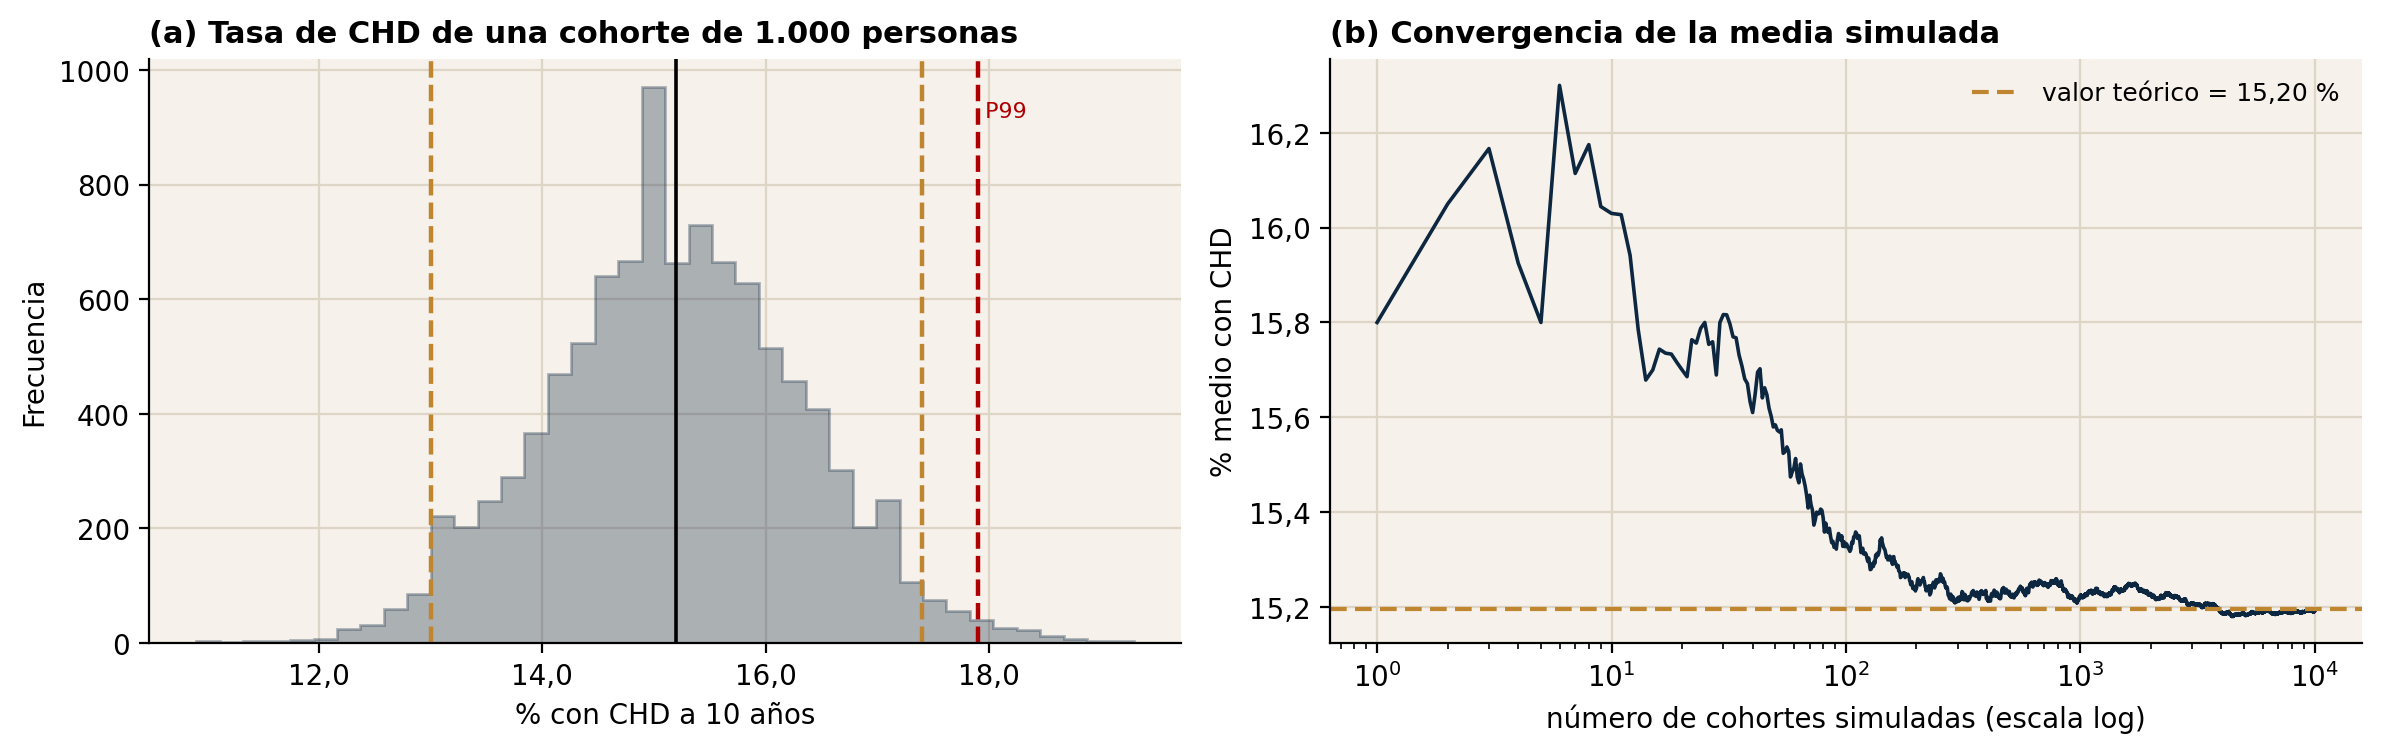
\includegraphics[width=\linewidth]{figuras/fig_montecarlo.png}
\caption{Simulación para $N=1.000$: distribución de la tasa de CHD (izquierda) y convergencia de la media acumulada (derecha).}
\label{fig:mc}
\end{figure}

\textbf{Convergencia.} Con $N=1.000$ la tasa media simulada es 15,19\,\% (teórica 15,20\,\%) y el error estándar de Monte Carlo es de solo 0,011 puntos porcentuales; la media acumulada queda dentro de $\pm0{,}05$ puntos del valor teórico desde la cohorte n.\textsuperscript{o} 1.743, así que 10.000 iteraciones son más que suficientes.

\textbf{Escenarios.} La Tabla~\ref{tab:mc} muestra cómo cambia la incertidumbre con el tamaño de la cohorte. En una cohorte de 1.000 personas la tasa de CHD varía entre 13,0\,\% y 17,4\,\% (IC 95\,\%) y solo en 0,5\,\% de las cohortes supera 18,2\,\% (tres puntos sobre lo esperado). Con $N=4.238$, el riesgo relativo simulado va de 1,96 a 2,60 (percentiles 2,5 y 97,5), prácticamente igual al IC de S1: la simulación reproduce la incertidumbre de los datos reales. En cohortes pequeñas, en cambio, la asociación hipertensión--CHD solo sería detectable en 42\,\% de los casos con $N=100$, con riesgos relativos entre 0,82 y 6,53: un estudio pequeño puede pasar por alto una asociación real o exagerarla.

\begin{table}[H]
\centering
\small
\caption{Resultados de la simulación según el tamaño de la cohorte.}
\label{tab:mc}
\begin{tabular}{rcccc}
\toprule
$N$ & Tasa CHD, IC 95\,\% (\%) & Ancho (pp) & RR P2,5--P97,5 & RR signif. (\%) \\
\midrule
100   & 9,0--23,0   & 14,0 & 0,82--6,53 & 42,2 \\
250   & 10,8--19,6  & 8,8  & 1,26--4,15 & 77,8 \\
500   & 12,2--18,4  & 6,2  & 1,49--3,43 & 96,7 \\
1.000 & 13,0--17,4  & 4,4  & 1,69--3,03 & 99,98 \\
4.238 & 14,1--16,3  & 2,2  & 1,96--2,60 & 100 \\
\bottomrule
\end{tabular}
\end{table}

\textbf{Limitación.} El escenario trata los tres parámetros como valores fijos e independientes entre personas, por lo que no propaga la incertidumbre con que S1 los estimó y subestima la variabilidad real.

% ===================================================================
% Responsable: Pablo Ríos
\section{Análisis de robustez}

Se evaluó la sensibilidad de S1 frente a valores extremos y supuestos con cuatro análisis, todos en el notebook.

\textbf{(a) Medias.} Recortar el 5\,\% de los casos extremos baja la media 3,1\,\% en la glucosa (de 81,97 a 79,44 mg/dL; 4,9\,\% de atípicos según Tukey, 1977), 0,6\,\% en el colesterol y 1,1\,\% en la presión sistólica; sin atípicos, la media de glucosa (78,49) se acerca a su mediana (78,0), por lo que para su valor típico conviene la mediana. En cambio, el error estándar no se mueve: el jackknife coincide con el clásico (glucosa 0,386; colesterol 0,689; presión sistólica 0,339) y la observación más influyente cambia la media en solo 0,08, 0,11 y 0,04 unidades (hasta 0,2 errores estándar).

\textbf{(b) Correlaciones.} Al excluir los atípicos de Tukey, presión sistólica con CHD baja de 0,22 a 0,18 (126 filas excluidas) y presión sistólica con diastólica de 0,78 a 0,75 (162 filas); las de hipertensión con presión sistólica y de edad con CHD no cambian. Ninguna fila individual altera una correlación en más de 0,003 (jackknife): no hay un caso dominante, pero el conjunto de extremos sí infla algo la relación entre presión sistólica y CHD.

\textbf{(c) Prueba de edad.} t de Student ($p=6{,}8\times10^{-50}$), Welch ($1{,}0\times10^{-48}$), Mann--Whitney ($1{,}2\times10^{-47}$) y permutación ($<0{,}0001$) llevan a la misma decisión; la probabilidad de que una persona con CHD sea mayor que una sin CHD es 0,68. La conclusión no depende de la distribución supuesta.

\textbf{(d) Distribuciones alternativas.} Se simuló la cobertura del IC clásico de la media de glucosa (10.000 muestras por caso). Con una población lognormal con la media y desviación de S1, cubre entre 94,8\,\% y 95,2\,\% desde $n=30$ hasta 3.850. Con la distribución empírica de la glucosa (asimetría 6,2; curtosis en exceso 58,6, colas muy pesadas) la cobertura cae a 88,0\,\% con $n=30$ y 89,1\,\% con $n=100$, y sube a 93,5\,\% con $n=500$ y 94,5\,\% con $n=3.850$; además, los intervalos fallan casi siempre hacia abajo. El Teorema Central del Límite depende entonces del tamaño de muestra y del peso de las colas: con el $n$ de S1 el IC de glucosa es confiable, con muestras de 100 o menos habría sido demasiado optimista.

\textbf{Conclusiones.} \emph{Confiables:} los IC de edad, colesterol y presión sistólica medias y de la proporción de CHD; las dos pruebas de hipótesis; y las correlaciones presión sistólica--diastólica, hipertensión--presión sistólica y edad--CHD. \emph{Requieren cautela:} la media de glucosa como valor típico; la magnitud de las correlaciones con presión sistólica, que se atenúa sin atípicos; la correlación fumador--CHD, indistinguible de cero; y el IC de la mediana, toscamente discreto. \emph{Supuesto sin verificar:} la independencia entre participantes.

% ===================================================================
% Responsable: Pablo Ríos
\section{Preparación para la Sumativa 3}

La Tabla~\ref{tab:val} resume los resultados validados. El notebook los guarda, junto con las observaciones influyentes, en dos archivos CSV de la carpeta de la evaluación.

\begin{table}[H]
\centering
\small
\caption{Resultados de S1 validados con remuestreo (resumen).}
\label{tab:val}
\begin{tabular}{>{\raggedright\arraybackslash}p{5.6cm} >{\raggedright\arraybackslash}p{5.2cm} l}
\toprule
\textbf{Resultado de S1} & \textbf{Evidencia de S2} & \textbf{Veredicto} \\
\midrule
Edad, colesterol y presión sistólica medias; proporción de CHD & IC BCa entre 0,6\,\% y 1,4\,\% de amplitud del clásico & Robusto \\
Mediana del colesterol & IC percentil y BCa toscos (valores enteros) & Cautela \\
Edad y CHD (Welch); hipertensión y CHD ($\chi^2$) & $p$ de permutación $=0{,}0001$ en ambas & Robusto \\
Correlaciones PAS--PAD, hipertensión--PAS, edad--CHD & IC bootstrap sin el cero, estrechos & Robusto \\
Correlación fumador--CHD ($r=0{,}02$) & IC bootstrap incluye el cero & Inestable \\
\bottomrule
\end{tabular}
\end{table}

\textbf{Observaciones influyentes.} La fila 481 (mujer de 64 años, presión sistólica 295 mmHg, con CHD) influye en tres resultados; la 2909 (glucosa 394 mg/dL), la 3160 (colesterol 696 mg/dL), la 2197 y la 781 afectan uno cada una. Su efecto es pequeño, pero deben registrarse.

\textbf{Recomendaciones para S3.}
\begin{enumerate}[leftmargin=1.6em,itemsep=0.1em,topsep=0.2em]
\item \emph{Predictoras estables:} edad y presión sistólica tienen asociación estable con CHD ($r\approx0{,}22$). Hipertensión prevalente y presión sistólica están muy correlacionadas ($r\approx0{,}70$): elegir una o verificar el VIF si van juntas.
\item \emph{Tabaquismo:} su correlación marginal con el CHD no se distingue de cero; eso no permite descartarlo en un modelo multivariable, donde debe evaluarse.
\item \emph{Valores extremos:} no eliminarlos, por ser clínicamente plausibles (S1). Para la glucosa conviene una transformación logarítmica o acotar al percentil 99.
\item \emph{Observaciones influyentes:} ajustar los modelos con y sin las filas listadas y reportar si cambian los coeficientes.
\item \emph{Incertidumbre del desempeño:} con 15,2\,\% de prevalencia, un conjunto de prueba del 30\,\% tiene unos 190 casos de CHD; usar partición estratificada, validación cruzada repetida e IC bootstrap para AUC, sensibilidad y precisión.
\item \emph{Faltantes:} la glucosa (9,2\,\%) es la que más tiene; imputar con la mediana calculada solo en el conjunto de entrenamiento para no filtrar información.
\end{enumerate}

% ===================================================================
% Responsable: Pablo Ríos
\section{Bibliografía (APA 7)}

\begin{list}{}{\leftmargin=1.5em \itemindent=-1.5em \itemsep=0.05em \parsep=0pt}\footnotesize\raggedright
\item Dileep. (s.f.). \textit{Heart disease prediction using logistic regression} [Conjunto de datos]. Kaggle. \url{https://www.kaggle.com/datasets/dileep070/heart-disease-prediction-using-logistic-regression}
\item Efron, B. (1987). Better bootstrap confidence intervals. \textit{Journal of the American Statistical Association, 82}(397), 171--185. \url{https://doi.org/10.1080/01621459.1987.10478410}
\item Efron, B., \& Tibshirani, R. J. (1993). \textit{An introduction to the bootstrap}. Chapman \& Hall.
\item Fisher, R. A. (1915). Frequency distribution of the values of the correlation coefficient in samples from an indefinitely large population. \textit{Biometrika, 10}(4), 507--521. \url{https://doi.org/10.2307/2331838}
\item Harris, C. R., Millman, K. J., van der Walt, S. J., Gommers, R., Virtanen, P., Cournapeau, D., Wieser, E., Taylor, J., Berg, S., Smith, N. J., Kern, R., Picus, M., Hoyer, S., van Kerkwijk, M. H., Brett, M., Haldane, A., Fernández del Río, J., Wiebe, M., Peterson, P., \dots\ Oliphant, T. E. (2020). Array programming with NumPy. \textit{Nature, 585}(7825), 357--362. \url{https://doi.org/10.1038/s41586-020-2649-2}
\item Maidana, J. P. (2026). \textit{Bootstrap para intervalos de confianza} [Apunte de clase]. MCDI501: Estadística Computacional para la Toma de Decisiones, Universidad Andrés Bello.
\item McKinney, W. (2010). Data structures for statistical computing in Python. En \textit{Proceedings of the 9th Python in Science Conference} (pp.~56--61). \url{https://doi.org/10.25080/Majora-92bf1922-00a}
\item Morris, T. P., White, I. R., \& Crowther, M. J. (2019). Using simulation studies to evaluate statistical methods. \textit{Statistics in Medicine, 38}(11), 2074--2102. \url{https://doi.org/10.1002/sim.8086}
\item Phipson, B., \& Smyth, G. K. (2010). Permutation P-values should never be zero: Calculating exact P-values when permutations are randomly drawn. \textit{Statistical Applications in Genetics and Molecular Biology, 9}(1), Artículo 39. \url{https://doi.org/10.2202/1544-6115.1585}
\item Tukey, J. W. (1977). \textit{Exploratory data analysis}. Addison-Wesley.
\item Virtanen, P., Gommers, R., Oliphant, T. E., Haberland, M., Reddy, T., Cournapeau, D., Burovski, E., Peterson, P., Weckesser, W., Bright, J., van der Walt, S. J., Brett, M., Wilson, J., Millman, K. J., Mayorov, N., Nelson, A. R. J., Jones, E., Kern, R., Larson, E., \dots\ SciPy 1.0 Contributors. (2020). SciPy 1.0: Fundamental algorithms for scientific computing in Python. \textit{Nature Methods, 17}(3), 261--272. \url{https://doi.org/10.1038/s41592-019-0686-2}
\item Welch, B. L. (1947). The generalization of ``Student's'' problem when several different population variances are involved. \textit{Biometrika, 34}(1--2), 28--35. \url{https://doi.org/10.1093/biomet/34.1-2.28}
\item Whelton, P. K., Carey, R. M., Aronow, W. S., Casey, D. E., Jr., Collins, K. J., Dennison Himmelfarb, C., DePalma, S. M., Gidding, S., Jamerson, K. A., Jones, D. W., MacLaughlin, E. J., Muntner, P., Ovbiagele, B., Smith, S. C., Jr., Spencer, C. C., Stafford, R. S., Taler, S. J., Thomas, R. J., Williams, K. A., Sr., \dots\ Wright, J. T., Jr. (2018). 2017 ACC/AHA/AAPA/ABC/ACPM/AGS/APhA/ASH/ASPC/NMA/PCNA guideline for the prevention, detection, evaluation, and management of high blood pressure in adults. \textit{Hypertension, 71}(6), e13--e115. \url{https://doi.org/10.1161/HYP.0000000000000065}
\end{list}

\end{document}
